\chapter{Simulador de radiología diagnóstica} 
\label{cap:xray}

 

%En este capítulo, se va a mostrar otro caso de uso en esta tesis.  El algoritmo propuesto permite modificar la posición de un paciente virtual interactivamente y es posible incorporarlo en cualquier simulador que requiera una adaptación del modelo en tiempos interactivos. 



En el contexto de la enseñanza de radiología diagnóstica, existen métodos de aprendizaje para ayudar al estudiante de radiología (ver sec, \ref{art:xraysim}), pero se han encontrado las siguientes limitaciones:

\begin{itemize}
\item Principalmente, los profesores usan repetidamente las mismas imágenes estáticas en sus clases, presentando el mismo caso una y otra vez.
\item No se pueden conseguir nuevas imágenes médicas instantáneamente para las clases.
\item No es posible variar la configuración de la anatomía mostrada ni conseguir diferentes anatomías para una misma configuración.
\item ProjectionVR$^{TM}$\cite{shanahan2016student} y \emph{medspace.VR} \cite{medspace} son simuladores para practicar el procedimiento en radiología diagnóstica, pero sus ejemplos son limitados.
\end{itemize}

Con estas limitaciones, en este capítulo se ha propuesto crear un simulador de radiología diagnóstica que pueda suplir las carencias antes citadas. Las herramientas de \ac{RV} permiten entrenar procedimientos médicos en un entorno seguro. Sobre todo, esto se vuelve especialmente importante si el entorno de trabajo no es seguro ni para pacientes ni para los propios profesionales, evitando en este caso radiaciones peligrosas para la salud. Sin necesidad de pacientes reales, y sin límites de tiempo, estudiantes y profesores serán capaces de revisar numerosos de casos diferentes, con la posibilidad de probar infinidad de configuraciones de la máquina de rayos X, e incluso, pudiendo trabajar con ejemplos incorrectos que no son habitualmente mostrados en la formación clásica.

%Por tanto, un simulador de \ac{RV} puede ayudar a mejorar el proceso de aprendizaje de los estudiantes de radiología. 

En colaboración con el Dr. Franck P. Vidal, se ha desarrollado un simulador de radiología diagnóstica.  %El algoritmo será el encargado de modificar el paciente virtual  mientras que la librería \emph{gVirtualXray}\cite{sujar:hal} proporciona una imagen simulada de rayos X, todo esto  en tiempo real.
%Comentar cosas de aprendizaje por la cual necesitamos un simulador
Este contará con la capacidad de generar variabilidad anatómica del algoritmo propuesto en esta tesis. Este simulador ha sido diseñado para ser flexible con el objetivo de introducir la mayor cantidad de pacientes virtuales externos. La herramienta \ac{TPTVPH} permite trabajar con modelos anatómicos incompletos y sin descripciones mecánicas, siendo únicamente estar presente los tejidos óseos y la piel (ver sec. \ref{posing:req}). El usuario podrá modificar interactivamente la anatomía del paciente virtual con la finalidad de mover al paciente a las proyecciones radiológicas con una modificación de la herramienta \ac{TPTVPH}. A su vez, la librería \emph{gVirtualXray}\cite{sujar:hal}  permitirá simular imágenes radiológicas del modelo anatómico en tiempo real. El módulo \ac{Courseware} integrará las dos tecnologías, permitiendo crear un simulador que contribuya a mejorar el entrenamiento de radiólogos noveles.



\section{Descripción del simulador} 
\label{xray:method}

%La combinación del algoritmo propuesto en esta tesis, y la librería que permite simular rayos X permite crear un simulador para entrenar proyecciones radiológicas.
%El simulador de radiología diagnóstica permitirá a estudiantes y profesores manipular cualquier variación de anatomía humana (ver sección \ref{posing:req}) y configurar la maquina de rayos X virtual para obtener de manera inmediata una radiografía simulada. Estudiantes y profesores pueden dedicar todo el tiempo necesario en una herramienta interactiva sin riesgo ninguno frente a la práctica en un entorno real.

El simulador de radiología diagnóstica se compone de tres módulos diferenciados: la herramienta \ac{TPTVPH}, la librería \emph{gVirtualXray} y un \ac{Courseware}.
En este sentido, el usuario podrá cargar cualquier modelo (previamente de ejecutar el proceso previo explicado en la sec. \ref{posing:preprocess}) y  posicionar el paciente virtual junto con su anatomía interna (ver sec. \ref{posing:Poses}) gracias a \ac{TPTVPH}. Por otra parte, con la librería \emph{gVirtualXray} se podrá configurar los parámetros del simulador de rayos X (ver sec. \ref{xray:setupxray}) y mientras muestra la imagen radiográfica en tiempo real. Por último, se ha desarrolla un módulo \ac{Courseware} que permite al usuario practicar el procedimiento completo.


%El módulo \ac{Courseware} presentan en una  Por una parte, podrá observar la representación 3D de las mallas superficiales cargadas a la vez que podrá observar la imagen de rayos X en todo momento, resultado de la proyección del emisor al detector. %Esta proyección podrá ser modificada por el usuario a través del ratón o los botones diseñados para tal efecto.
El \ac{Courseware} se ha desarrollado con la finalidad de integrar las dos herramientas y crear una interfaz donde el usuario podrá interaccionar con el simulador y la funcionalidad de herramienta de aprendizaje.
Los usuarios revisar multitud de escenarios, probar parámetros concretos de la maquina de rayos x, focalizarse en errores comunes que se realizan en los entornos reales o enfatizar en pequeños detalles. Además, se puede variar la anatomía del paciente virtual y parámetros que no es posible en los archivos educativos donde solo se encuentran imágenes estáticas. El objetivo final es mejorar la confianza de los futuros profesionales médicos con vistas a reducir la dosis y el número de repeticiones que sufrirán los pacientes. Aunque las dos tecnologías son computacionalmente intensas, se ha aprovechado de las capacidades de la arquitectura de las tarjetas gráficas. Ambas librerías trabajan sobre el mismo conjunto de datos al compartir memoria en \acs{GPU}, por lo cual la comunicación es inmediata.

En cuanto a la arquitectura de este simulador, citando la definición de \emph{Burdea y Coiffet} vista en la sección \ref{art:simulador}, se ha descrito los módulos que corresponden al motor de \ac{RV} y al software. En este caso, los dispositivos de \ac{E/S} son el monitor, teclado y ratón. En la figura \ref{fig:Posesummary} muestra la arquitectura del simulador. El preproceso toma el modelo anatómico como entrada para generar las estructuras necesarias que permiten a la selección de poses ejecutarse interactivamente. El \ac{Courseware} integra las dos librerías y muestra el paciente virtual a través de la interfaz de usuario.

\begin{figure}[h]
\centering
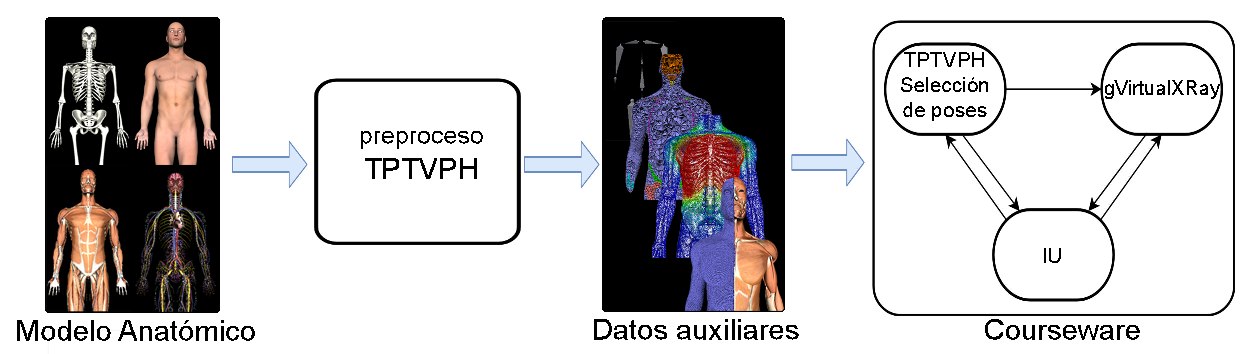
\includegraphics[width=\linewidth]{IMG/ArquXRAY.pdf}

\caption{\label{fig:Posesummary} Arquitectura del simulador: i) modelos anatómicos de entrada ii) Proceso previo ejecutado una vez por paciente virtual iii) Datos generados necesarios para TPTVPH iv) \ac{Courseware} donde se ha integra la \emph{selección de poses} con \emph{gVirtualXRay}.
}
\end{figure}

A continuación se va a introducir la librería \emph{gVirtualXRay} y después se pasará a describir el desarrollo realizado en el \ac{Courseware}


\section{gVirtualXray}
\label{xray:context}

Una de las principales características de la librería \emph{gVirtualXray} es la capacidad de simular imágenes realistas de rayos X en tiempo real. La interacción es una cualidad fundamental en cualquier simulador de \ac{RV}, por lo que esta librería es perfecta para la creación de una aplicación de diagnóstico por imagen. 
A su vez, la librería utiliza la representación superficial de triángulos, habitualmente usada en gráficos por computador, y compatible con la herramienta \ac{TPTVPH}.

\emph{gVirtualXray} implementa la técnica de trazador de rayos propuesta en \cite{Freud2006175}, llamada \emph{L-buffer}. En este método, utilizando las capacidades de la \ac{GPU}, se calcula la longitud de los rayos X que pasan a través de la malla poligonal, desde la posición del emisor de rayos X hasta cada \emph{píxel} del detector. En la intersección rayo-polígono se resuelve la ley de \emph{Beer-Lambert}. Esto permite la posibilidad de simular eficientemente las imágenes de rayos X de cualquier superficie poligonal utilizando el cauce gráfico. La ecuación \emph{Beer-Lambert} se resuelve para cada punto de la imagen simulada, donde se relaciona la absorción de la luz (en este caso fotones) con las propiedades del material.  Se utiliza la \emph{Photon Cross Sections Database (XCOM)} creada por \emph{National Institute of Standards and Technology (NIST)}\cite{XCOM} como referencia para calcular el coeficiente de atenuación másico. Esto da como resultado la posibilidad de generar imágenes visualmente realistas de radiografías y fluoroscópicas. Para más información se puede consultar \cite{vidal2009simulation}.

Esta técnica permite la simulación en tasa de refresco interactivas, en comparación con las técnicas de  simulación de \emph{Monte Carlo}, más habitual en la bibliografía \cite{sujar:hal}. La fidelidad de las imágenes resultantes (Fig. \ref{fig:validation}), se han validado usando \emph{Geant4}, una herramienta desarrollada por el \emph{European Organization for Nuclear Research (CERN)} que se encuentra como referencia en el estado del arte de la simulación de rayos X.

\begin{figure}[h]
    \begin{subfigure}[b]{0.25\linewidth}
        \centering
        {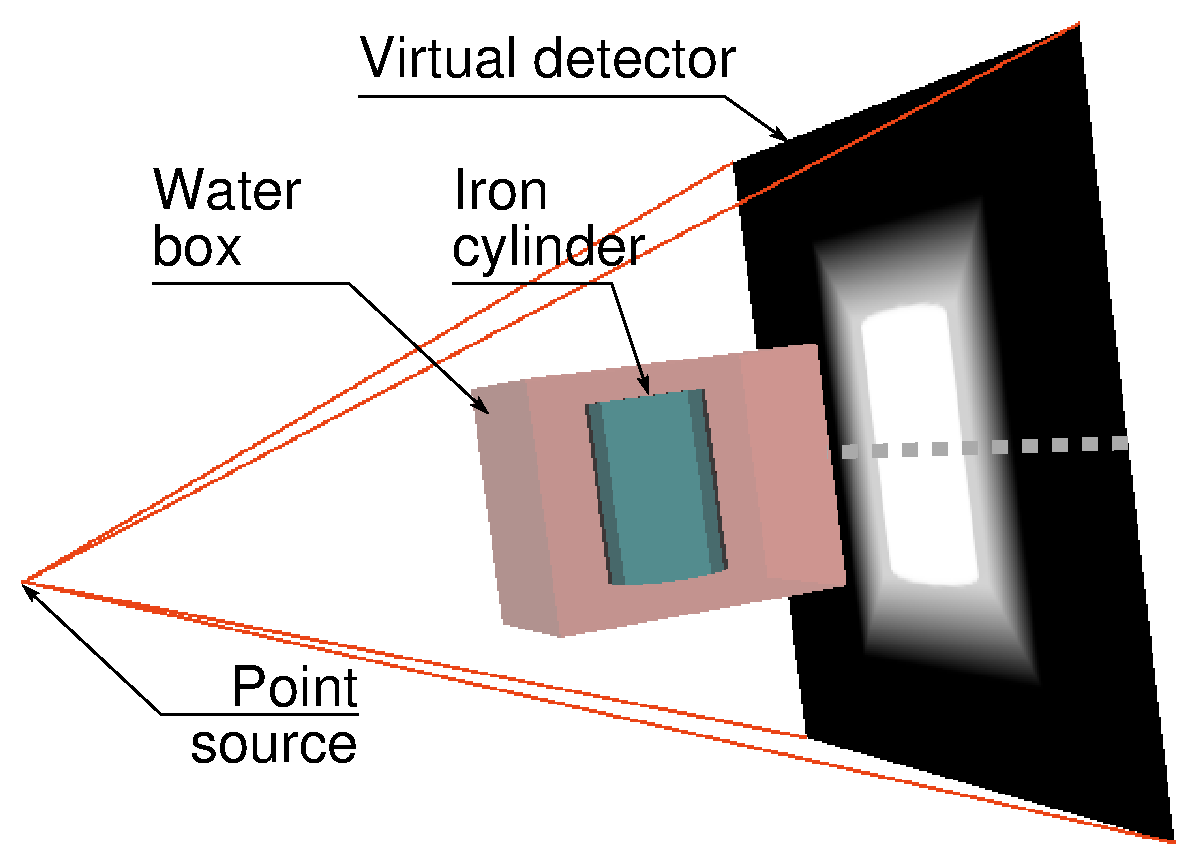
\includegraphics[width=0.8\linewidth]{IMG/figure3a.eps}}
        \caption{\label{subfig:polychromatismA} Escena de prueba.}
    \end{subfigure}
    \null\hfill
     \begin{subfigure}[b]{0.25\linewidth}
        \centering
        {\includegraphics[width=\linewidth]{IMG/figure6a.eps}}
        \caption{\label{subfig:GPU} Imagen determinista simulada  usando \emph{gVirtualXRay}.}
    \end{subfigure}
    \null\hfill
    \begin{subfigure}[b]{0.25\linewidth}
        \centering
        {\includegraphics[width=\linewidth]{IMG/figure6b.eps}}
        \caption{\label{subfig:Gate} Imagen simulada utilizando \emph{Monte Carlo} en \emph{Geant4}.}
    \end{subfigure}

\caption{\label{fig:validation} Ejemplo de la evaluación para la herramienta \emph{gVirtualXRay} \cite{sujar:hal}.}
\end{figure}











